% THIS TEMPLATE IS A WORK IN PROGRESS

\documentclass[polish, a4paper]{article}
\usepackage[a4paper,left=4cm,right=4cm,top=2.5cm,bottom=2.5cm]{geometry}
\usepackage[T1]{fontenc}
\usepackage[polish]{babel}
\usepackage[utf8]{inputenc}
\usepackage{hyperref}
\usepackage{fancyhdr}
\usepackage{float}
\usepackage{graphicx}
\usepackage{titling}
\usepackage{caption}
\usepackage{pgfplots}
\usepackage{pgfplotstable}
\usepackage{filecontents}
\graphicspath{ {./} }
\pagestyle{fancy}

\setlength{\droptitle}{-1in}

%\lhead{\includegraphics[width=0.2\textwidth]{nyush-logo.pdf}}

  \lhead{Maciej Kaszkowiak}
  \chead{Ćwiczenie 225}
  \rhead{Lab 4,
  151856}


%%%% PROJECT TITLE
\title{Badanie właściwości dielektrycznych ciał stałych\\
        \Large \emph{Ćwiczenie nr 225 z działu Elektromagnetyzm}}

%%%% NAMES OF ALL THE STUDENTS INVOLVED (first-name last-name)
\author{Maciej Kaszkowiak, Lab 4, 151856}

\date{\vspace{-5ex}} %NO DATE


\begin{document}
\maketitle
%\thispagestyle{titlepage}

\section{Cel ćwiczenia}
Przeprowadzone ćwiczenie ma dwa główne cele:
\begin{enumerate}
\item{Zbadanie zależności pojemności płaskiego kondensatora powietrznego od
odległości między jego okładkami.}
\item{Wyznaczenie przenikalności elektrycznej oraz tangensa kąta strat (współczynnika stratności) wybranych dielektryków.}
\end{enumerate}
\section{Wstęp teoretyczny}


W doświadczeniu wykorzystano kondensator płaski, który składa się z dwóch okładek wykonanych z przewodnika. Gdy kondensator jest podłączony do zewnętrznego źródła napięcia, na okładkach pojawiają się ładunki różnoimienne o tej samej wartości. W ten sposób między okładkami powstaje pole elektryczne.

\begin{equation}
E_{wyp} = E_0 - E_{ind}
\end{equation}

Jeżeli między okładki kondensatora włożymy płytkę wykonaną z dielektryka, to pole elektryczne występujące w kondensatorze zostanie zmniejszone przez indukowane pole elektryczne wytworzone przez dielektryk (ze względu na zjawisko polaryzacji).


\begin{figure}[H]
\centering
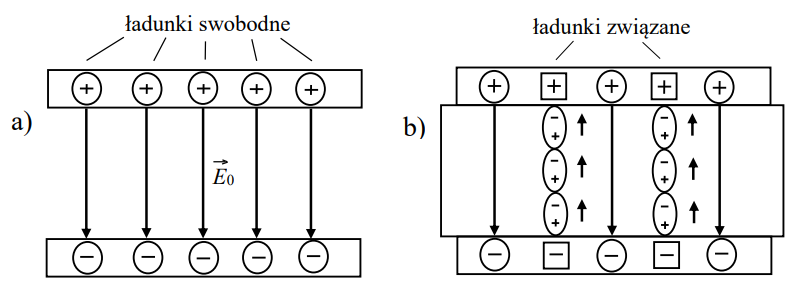
\includegraphics[width=0.6\textwidth]{kondensator.png}
\caption{a) kondensator próżniowy, b) kondensator z dielektrykiem}
\end{figure}

Pojemność kondensatora jest proporcjonalna do powierzchni okładek kondensatora i odwrotnie proporcjonalna do odległości między okładkami. Na pojemność kondensatora proporcjonalnie wpływają również stała przenikalności elektrycznej próżni $\epsilon_0$ oraz względna przenikalność elektryczna dielektryka $\epsilon_r$.


\begin{equation}
C_0 = \epsilon_0 \frac{S}{d} < C = \epsilon_0 \epsilon_r \frac{S}{d}
\end{equation}
\section{Przebieg ćwiczenia}

\begin{enumerate}
\item {Uruchomiliśmy miernik Escort ELC-3131D. Ustawiliśmy parametry pomiarowe - zakres automatyczny, pomiar pojemności, częstotliwość pomiarowa: 1 kHz.}
\item {Wykonaliśmy serię 18 pomiarów pojemności kondensatora, zmieniając odległość d między okładkami kondensatora w zakresie od 0.2 do 5 cm.}
\item {Wykonaliśmy serię 4 pomiarów dla czterech wybranych dielektryków. Po umieszczeniu dielektryka między okładkami kondensatora zanotowaliśmy odległość pomiędzy okładkami (dokładność: 0,1 mm), pojemność, dobroć oraz tangens kąta strat.}
\item {Po wykonaniu pomiaru dla każdego z dielektryków powtórzyliśmy pomiary dla kondensatora powietrznego przy zachowaniu tej samej odległości między okładkami.}
\end{enumerate}

\begin{figure}[H]
\centering
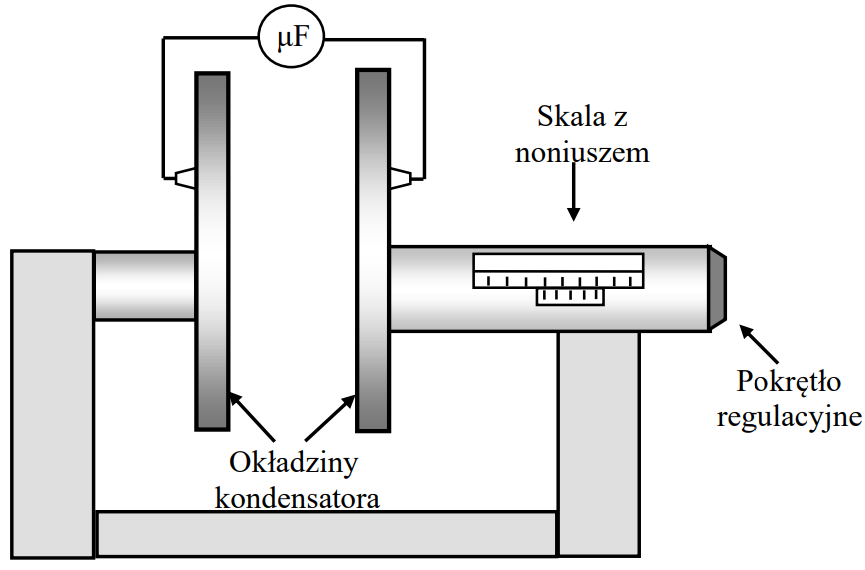
\includegraphics[width=0.4\textwidth]{kondensator pomiarowy.png}
\caption{Kondensator pomiarowy}
\end{figure}

\section{Wyniki pomiarów}

Pomiary odległości zostały wykonane z dokładnością do 0,1 mm z wykorzystaniem noniusza. Pomiary pojemności zostały wykonane z dokładnością do 0,1 pF. Pomiar dobroci został wykonany z dokładnością do 0,1 wielkości, natomiast pomiar tangensa kąta strat został wykonany z dokładnością do 0,001 wielkości.
\begin{table}[H]
    \centering
    \captionsetup{justification=centering}
    \begin{tabular}{|c|c|c|c|}
    \hline
        \textbf{Nr pomiaru} & \textbf{Odległość} & \textbf{Odwrotność odległości} & \textbf{Pojemność} \\
        & \textbf{[mm]} & \textbf{[1/mm]} & \textbf{[pF]} \\ \hline
        1 & 2,0 & 0,5000 & 281,5 \\ \hline
        2 & 3,0 & 0,3333 & 191,6 \\ \hline
        3 & 4,0 & 0,2500 & 149,2 \\ \hline
        4 & 5,0 & 0,2000 & 122,6 \\ \hline
        5 & 6,0 & 0,1667 & 106,6 \\ \hline
        6 & 7,0 & 0,1429 & 93,2 \\ \hline
        7 & 8,0 & 0,1250 & 86,6 \\ \hline
        8 & 9,0 & 0,1111 & 78,5 \\ \hline
        9 & 10,0 & 0,1000 & 75,3 \\ \hline
        10 & 12,0 & 0,0833 & 65,1 \\ \hline
        11 & 15,0 & 0,0667 & 59,9 \\ \hline
        12 & 17,0 & 0,0588 & 57,6 \\ \hline
        13 & 20,0 & 0,0500 & 55,2 \\ \hline
        14 & 25,0 & 0,0400 & 53,0 \\ \hline
        15 & 30,0 & 0,0333 & 51,4 \\ \hline
        16 & 35,0 & 0,0286 & 50,1 \\ \hline
        17 & 42,0 & 0,0238 & 47,1 \\ \hline
        18 & 50,0 & 0,0200 & 46,0 \\ \hline
    \end{tabular}
        \caption{Seria 18 pomiarów pojemności kondensatora próżniowego ze zmienną odległością w zakresie 2-50mm}
\end{table}

\begin{table}[H]
    \centering
    \captionsetup{justification=centering}
    \begin{tabular}{|c|c|c|c|c|c|}
    \hline
        \textbf{Nr} & \textbf{Materiał} & \textbf{Odległość} & \textbf{Pojemność} & \textbf{Dobroć} & \textbf{Tangens} \\ 
        \textbf{próbki}& & & \textbf{[pF]} & \textbf{Q} & \textbf{kąta strat}
        \\ \hline
        1 & Akrylit & 4,9 mm & 302,9 & 25,8 & 0,038 \\ 
        1p & Powietrze & 4,9 mm & 125,6 & - & - \\ \hline
        2 & ? & 9,9 mm & 175,2 & 62,1 & 0,015 \\ 
        2p & Powietrze & 9,9 mm & 71,7 & - & - \\ \hline
        3 & Plexiglass & 11,0 mm & 161,4 & 19,3 & 0,051 \\ 
        3p & Powietrze & 11,0 mm & 67,4 & - & - \\ \hline
        4 & ? & 10,4 mm & 162,4 & 23,8 & 0,041 \\ 
        4p & Powietrze & 10,4 mm & 69,9 & - & - \\ \hline
    \end{tabular}
    \caption{Seria 4 pomiarów dla czterech różnych dielektryków oraz 4 pomiarów dla kondensatorów próżniowych zgodnych odległością pomiędzy okładkami}
\end{table}
\section{Opracowanie wyników}
\subsection{Zbadanie zależności pojemności płaskiego kondensatora powietrznego od odległości między jego okładkami}
Posłużyłem się wzorem wyznaczającego pojemność kondensatora powietrznego, gdzie $\epsilon_r = 1,0059$ wyznacza przenikalność dla powietrza znajdującego się pomiędzy okładkami.

\begin{equation}
C_0 = \epsilon_0 \epsilon_r \frac{S}{d}
\end{equation}
\begin{equation}
C_0 = \epsilon_0 \epsilon_r S \frac{1}{d}
\end{equation}

Przewody pomiędzy kondensatorem a miernikiem mogą posiadać niezerową pojemność, co należy uwzględnić w obliczeniach:

\begin{equation}
C_0 = \epsilon_0 \epsilon_r S \frac{1}{d} + C_p
\end{equation}

Zależność $C_0 = f(\frac{1}{d})$ można przedstawić w postaci funkcji liniowej $C_0 = a\frac{1}{d} + b$, 
traktując $\epsilon_0\epsilon_rS$ jako współczynnik kierunkowy $a$ oraz $C_p$ jako wyraz wolny $b$.

Z pomiarów dla kondensatora powietrznego wykonałem wykres $C_0 = f(\frac{1}{d})$.
Wykorzystując regresję liniową obliczyłem współczynnik kierunkowy prostej $a$ i wartość b punktu przecięcia z osią y. Wartość b jest równa pojemności przewodów łączących kondensator z miernikiem pomiarowym.

\begin{figure}[H]
\centering
\begin{tikzpicture}
\begin{axis}[
    width=\textwidth, height=0.5\textwidth,
    grid=major,
    xlabel={Odwrotność odległości 1/d (1/m)},
    ylabel={Pojemność (pF)}
]
\addplot[
    thick,
    orange
] table[
    x = d, col sep=comma,
    y = {create col/linear regression={y=C}}
] {wykres1.csv};
\addplot table[teal, only marks, x=d, y=C, col sep=comma] {wykres1.csv};
\end{axis}
\end{tikzpicture}
\caption{Wykres zależności pojemności kondensatora od odwrotności odległości pomiędzy jego okładkami.}
\end{figure}

Z wykorzystaniem kalkulatora \emph{Statystyka pomiarów} autorstwa Stanisława Szuby 
ustaliłem współczynniki $a$, $b$ oraz $R^2$ z wykorzystaniem regresji liniowej.

\begin{equation}
a = 0,486 \;[pF \cdot m]
\end{equation}
\begin{equation}
b = 29,741 \; [pF]
\end{equation}
\begin{equation}
R^2 = 0,9938
\end{equation}

Współczynnik $b = 29,741 \; [pF]$ wyznacza pojemność przewodów pomiędzy kondensatorem a miernikiem.
Na podstawie wyznaczonego współczynniku $a = \epsilon_0\epsilon_rS$ można ustalić przenikalność elektryczną próżni.

\begin{equation}
a = \epsilon_0\epsilon_rS
\end{equation}
\begin{equation}
\epsilon_0 = \frac{a}{S\epsilon_r}
\end{equation}
\begin{equation}
\epsilon_0 = \frac{0,486 \cdot 10^{-12}}{\pi \cdot (0,13)^2 \cdot 1,0059}
\end{equation}
\begin{equation}
\epsilon_0 = 9,10 \cdot 10^{-12} \; [\frac{F}{m}]
\end{equation}

W celu wyznaczenia niepewności pomiarowej wykorzystałem odchylenie standardowe współczynnika a, wyznaczone na podstawie wspołczynnika $R^2$.

\begin{equation}
\sigma_a = a - aR^2
\end{equation}
\begin{equation}
\sigma_a = 0,486 - 0,486 \cdot 0,9938
\end{equation}
\begin{equation}
\sigma_a = 0,003 \; [pF \cdot m]
\end{equation}

Następnie skorzystałem z różniczki logarytmicznej.

\begin{equation}
\epsilon_0 = \frac{S}{a}
\end{equation}
\begin{equation}
\Delta\epsilon_0 = \left\| - \frac{\Delta a}{a} \right\| \cdot \epsilon_0
\end{equation}
\begin{equation}
\Delta\epsilon_0 = \left\| - \frac{0,003 \cdot 10^{-12} }{0,486 \cdot 10^{-12}} \right\| \cdot 9,15 \cdot 10^{-12}
\end{equation}
\begin{equation}
\Delta\epsilon_0 = 0,0564 \cdot 10^{-12} [\frac{F}{m}]
\end{equation}

Tym samym, przenikalność próżni $\epsilon_0$ wynosi $9,10 \pm 0,06 \; [\frac{pF}{m}]$.
Wyznaczona wartość odbiega od wartości z tablic $\epsilon_0 = 8,854 \; [\frac{pF}{m}]$. Powodem źle wykonanych pomiarów może być błąd paralaksy przy ustalaniu odległości oraz niedokładny pomiar wynikający z długiego czasu stabilizacji przy pomiarze pojemności kondensatora.
\subsection{Wyznaczenie przenikalności elektrycznej oraz tangensa kąta strat (współczynnika stratności) wybranych dielektryków.}

W celu wyznaczenia rzeczywistej składowej względnej przenikalności elektrycznej danych dielektryków
posłużyłem się następującym wzorem:
\begin{equation}
\epsilon_r ' = \frac{C - C_p}{C_0 - C_p}
\end{equation}

gdzie $C$ to pojemność kondensatora z dielektrykiem, 
$C_0$ to pojemność kondensatora powietrznego, a $C_p$ to wcześniej wyznaczona pojemność przewodów.


Niepewności $\Delta C = \Delta C_0 = 0,1 \; pF$ biorą się z niepewności miernika, natomiast 
niepewność $\Delta C_p = 1,72 \; pF$ została odczytana z \emph{Kalkulatora pomiarów}.

Niepewność dla zmiennej $\epsilon_r'$ obliczyłem za pomocą metody różniczki całkowitej.

\begin{equation}
\Delta \epsilon_r' = 
\left\| \Delta C \frac{\delta}{\delta C} \right\| +
\left\| \Delta C_0 \frac{\delta}{\delta C_0}  \right\| + 
\left\| \Delta C_p \frac{\delta}{\delta C_p}  \right\|
\end{equation}


\begin{equation}
\frac{\delta}{\delta_C} 
= 
\frac{1}{C_0 - C_p} 
\end{equation}

\begin{equation}
\frac{\delta}{\delta_C_0} 
= 
\frac{C_p - C}{(C_0 - C_p)^2} 
\end{equation}

\begin{equation}
\frac{\delta}{\delta_C_p} 
= 
\frac{C - C_0}{(C_0 - C_p)^2} 
\end{equation}

Wyniki dla wszystkich 4 próbek zapisałem w poniższej tabeli.
\begin{table}[H]
    \centering
    \begin{tabular}{|c|c|c|}
    \hline
        \textbf{Nr próbki} & \textbf{$\epsilon'_r$} & \textbf{Niepewność} \\ \hline
        1 & 2,85 & 0,04 \\ \hline
        2 & 3,47 & 0,11 \\ \hline
        3 & 3,5 & 0,13 \\ \hline
        4 & 3,3 & 0,11 \\ \hline
    \end{tabular}
    \caption{Względna przenikalność elektryczna wraz z niepewnością dla poszczególnych próbek.}
\end{table}


Na podstawie zmierzonej dobroci oraz 
wyliczonej rzeczywistej składowej względnej przenikalności elektrycznej
mogę ustalić współczynnik strat $\epsilon_r''$, czyli zespoloną względną przenikalność elektryczną dielektryka.


\begin{equation}
Q = \frac{\epsilon'_r}{\epsilon''_r}
\end{equation}

\begin{equation}
\epsilon_r'' = \frac{\epsilon'_r}{Q}
\end{equation}

Wyniki dla wszystkich 4 próbek zapisałem w poniższej tabeli.

\begin{table}[H]
    \centering
    \begin{tabular}{|c|c|}
    \hline
        \textbf{Nr próbki} & \textbf{$\epsilon''_r$} \\ \hline
        1 & 0,11 \\ \hline
        2 & 0,06 \\ \hline
        3 & 0,18 \\ \hline
        4 & 0,14 \\ \hline
    \end{tabular}
    \caption{Współczynnik strat dla poszczególnych próbek}
\end{table}

Po przeprowadzeniu obliczeń mogę odczytać materiał próbek z wykorzystaniem następującej tabeli:

\begin{table}[H]
    \centering
    \begin{tabular}{|l|l|}
    \hline
        \textbf{Materiał} & $\epsilon_r$ \\ \hline
        Bakelit & 2,2-3,0 \\ \hline
        Ebonit & 2,0-3,5 \\ \hline
        Kwarc & 3-6 \\ \hline
        Pleksi & 3-3,7 \\ \hline
        Porcelana & 5,5-6,5 \\ \hline
        Powietrze & 1,0059 \\ \hline
        Szkło & 3,1-4,4 \\ \hline
        Tytanian strontu & 310 \\ \hline
    \end{tabular}
    \caption{Względna przenikalność elektryczna $\epsilon_r$ przykładowych materiałów dielektrycznych (t = 20°C)}
\end{table}

Materiał próbek przedstawia się następująco:

\begin{table}[H]
    \centering
    \begin{tabular}{|l|l|}
    \hline
        \textbf{Nr próbki} & \textbf{Ustalony materiał} \\ \hline
        1 & Akrylit \\ \hline
        2 & Bakelit \\ \hline
        3 & Plexiglass \\ \hline
        4 & Kwarc \\ \hline
    \end{tabular}
    \caption{Ustalony materiał poszczególnych próbek}
\end{table}

\section{Wnioski}

Przedstawione doświadczenie wykazało zależność liniową pomiędzy odwrotnością odległości pomiędzy okładkami kondensatora a pojemnością. Wykazałem również, że włożenie dielektryku pomiędzy okładki ma wpływ na pojemność zgodny z teoretycznymi wzorami. Przeprowadzone pomiary obarczone były niepewnością pomiarową, wynikającą z efektu paralaksy (dla pomiaru odległości pomiędzy okładkami) oraz z powolnej stabilizacji urządzenia służącego do pomiaru pojemności kondensatora. Ustaliłem materiał poszczególnych próbek dielektryków, lecz wynik przenikalności próżni $\epsilon_0$ nieznacznie odbiegł od założeń teoretycznych.    


\section{Bibliografia}

\begin{enumerate}
    \item {\emph{Badanie właściwości dielektrycznych ciał stałych} (Mirosław Szybowicz, Krzysztof Łapsa, Izabela Hanyż)}
    \item {\emph{Elektromagnetyzm. Ćwiczenie: 225. Badanie właściwości dielektrycznych ciał stałych.} (Krzysztof Łapsa) – film na platformie Youtube}
    \item {Kalkulator pomiarów: https://phys-old.put.poznan.pl/szuba/states/index.php}
\end{enumerate}


\end{document}
